\section{Vektorgeometrie}
\subsection{Definitionen}
\begin{itemize}
  \item Betrag eines Vektors -> Länge
  \item Vektor mit Betrag $0$ -> Nullvektor
  \item Vektor mit Betrag $1$ -> Einheitsvektor oder normiert
  \item $\lambda_1 \cdot \vec{a}_1 + \lambda_2 \cdot \vec{a}_2 + ... + \lambda_n \cdot \vec{a}_n$ -> Linearkombination
  \item Zwei Vektoren sind \textit{kollinear}, wenn es eine Gerade $g$ gibt, zu der beide parallel sind.
  \item Drei Vektoren sind \textit{komplanar}, wenn es eine Ebene gibt, zu der alle parallel sind.
  \item Linearkombination: $\vec{a} = a_1 \cdot \vec{e}_1 + a_2 \cdot \vec{e}_2$ diese reellen Zahlen heissen \textit{Komponenten} des Vektors $\vec{a}$ -> $\begin{pmatrix} a_1 \\ a_2 \end{pmatrix}$
  \item Zu jedem Punkt $P$ der Ebene bzw. des Raumes definieren wir den \textit{Ortsvektor} $\vec{r}(P)=\vec{OP}$
\end{itemize}

\subsection{Rechnen mit Vektoren}
\begin{center}
  \includegraphics[width=0.9\linewidth]{images/rechnen_vektor.png}
  \includegraphics[width=0.9\linewidth]{images/rechnen_vektor_zwei.png}
\end{center}

\subsection{Skalarprodukt}
\subsubsection{Definition Skalarprodukt}%
\label{ssub:Definition Skalarprodukt}
\begin{equation*}
  \vec{a} \cdot \vec{b} = |\vec{a}| \cdot |\vec{b}| \cdot \cos{\varphi}
\end{equation*}
Dabei ist $\varphi$ der Zwischenwinkel zwischen den Vektoren $\vec{a}$ und $\vec{b} (0 \leq \varphi \leq \pi)$
Wir definieren ausserdem: $\vec{a} \cdot \vec{0} = 0$, $\vec{0} \cdot \vec{b} = 0$

\subsubsection{Berechnung des Skalarproduktes aus der Komponentendarstellung der Vektoren}%
\label{ssub:Berechnung des Skalarproduktes aus der Komponentendarstellung der Vektoren}
\begin{center}
  \includegraphics[width=1\linewidth]{images/skalarpr.png}
\end{center}

\subsubsection{Satz}%
\label{ssub:Satz}
Für die orthogonale Projektion eines Vektors $\vec{b}$ auf einen Vektor $\vec{a}$ gilt:
\begin{equation*}
  \vec{b}_a = \frac{\vec{a} \cdot \vec{b}}{|\vec{a}|^2} \cdot \vec{a} \qquad |\vec{b}_a| = \frac{|\vec{a} \cdot \vec{b}|}{|\vec{a}|}
\end{equation*}

\subsection{Das Vektorprodukt}
\subsubsection{Definition}%
\label{ssub:Definition}
Das \textit{Vektorprodukt} $\vec{a} \times \vec{b}$ zweier räumlicher Vektoren $\vec{a}$ und $\vec{b}$ ist der eindeutig bestimmte Vektor mit folgenden Eigenschaften:
\begin{itemize}
  \item $|\vec{a} \times \vec{b}| = |\vec{a}| \cdot |\vec{b}| \cdot \sin{\varphi}$
  \item $\vec{a} \times \vec{b}$ ist orthogonal zu $\vec{a}$ und zu $\vec{b}$
  \item $\vec{a},\vec{b}$ und $\vec{a} \times \vec{b}$ bilden (in dieser Reihenfolge) ein Rechtssystem.
\end{itemize}
Dabei ist $\varphi$ der Zwischenwinkel zwischen $\vec{a}$ und $\vec{b} (0\leq \varphi \leq \pi)$. \\
Wir definieren ausserdem: $\vec{a} \times \vec{0} = \vec{0}, \vec{0} \times \vec{a} = \vec{0}$

\subsubsection{Berechnung des Vektorproduktes aus der Komponentendarstellung der Vektoren}%
\label{ssub:Berechnung des Vektorproduktes aus der Komponentendarstellung der Vektoren}
\begin{center}
  \includegraphics[width=0.6\linewidth]{images/berechnung_vektorprodukt.png}
\end{center}
\begin{center}
  \includegraphics[width=0.9\linewidth]{images/wichtige_eigenschaften_vektorprodukt.png}
\end{center}

\subsubsection{Fläche des aufgespannten Parallelogramms}%
\label{ssub:Fläche des aufgespannten Parallelogramms}
Der Betrag des Vektorproduktes $\vec{a} \times \vec{b}$ ist gleich dem Flächeninhalt des Parallelogramms, das von den Vektoren aufgespannt wird.

\tikzset{every picture/.style={line width=0.75pt}} %set default line width to 0.75pt        

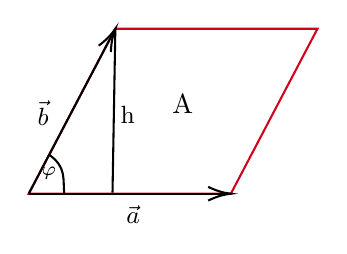
\begin{tikzpicture}[x=0.75pt,y=0.75pt,yscale=-1,xscale=1]
%uncomment if require: \path (0,300); %set diagram left start at 0, and has height of 300

%Shape: Parallelogram [id:dp14845767734072834] 
\draw  [color={rgb, 255:red, 208; green, 2; blue, 27 }  ,draw opacity=1 ] (104.74,29.5) -- (202.13,29.5) -- (160.39,109) -- (63,109) -- cycle ;
%Straight Lines [id:da47561790303627927] 
\draw    (63,109) -- (103.81,31.27) ;
\draw [shift={(104.74,29.5)}, rotate = 117.7] [color={rgb, 255:red, 0; green, 0; blue, 0 }  ][line width=0.75]    (10.93,-3.29) .. controls (6.95,-1.4) and (3.31,-0.3) .. (0,0) .. controls (3.31,0.3) and (6.95,1.4) .. (10.93,3.29)   ;
%Straight Lines [id:da27198439608244596] 
\draw    (63,109) -- (158.39,109) ;
\draw [shift={(160.39,109)}, rotate = 180] [color={rgb, 255:red, 0; green, 0; blue, 0 }  ][line width=0.75]    (10.93,-3.29) .. controls (6.95,-1.4) and (3.31,-0.3) .. (0,0) .. controls (3.31,0.3) and (6.95,1.4) .. (10.93,3.29)   ;
%Straight Lines [id:da24006701515558804] 
\draw    (104.74,29.5) -- (103.37,108.5) ;
%Curve Lines [id:da09890376474983598] 
\draw    (80.13,109) .. controls (79.38,102.25) and (81.38,96.25) .. (72.88,90.25) ;

% Text Node
\draw (67.75,94.75) node [anchor=north west][inner sep=0.75pt]  [font=\scriptsize] [align=left] {$\varphi$};
% Text Node
\draw (105.75,65.25) node [anchor=north west][inner sep=0.75pt]  [font=\small] [align=left] {h};
% Text Node
\draw (130.75,59.5) node [anchor=north west][inner sep=0.75pt]   [align=left] {A};
% Text Node
\draw (108.5,113.4) node [anchor=north west][inner sep=0.75pt]  [font=\small]  {$\vec{a}$};
% Text Node
\draw (65.75,62.9) node [anchor=north west][inner sep=0.75pt]  [font=\small]  {$\vec{b}$};


\end{tikzpicture}

\vfill

\subsection{Geraden und Ebenen}
\begin{center}
  \includegraphics[width=0.9\linewidth]{images/geraden1.png}
\end{center}
\begin{center}
  \includegraphics[width=0.9\linewidth]{images/geraden2.png}
\end{center}

\subsubsection{Schnittpunkte und Schnittgeraden}%
\label{ssub:Schnittpunkte und Schnittgeraden}
\textit{Schnittpunkt}: Punkt der auf allen beteiligten Geraden und Ebenen liegt. \\
\textit{Schnittgerade}: Besteht aus allen Punkten zweier Ebenen, die sowohl auf der einen als auch auf der anderen Ebene liegen. \\
\textit{Berechnung}: Aus den Gleichungen der beteiligten Geraden und Ebenen ein LGS aufstellen und dieses auflösen.

\subsubsection{Abstände}%
\label{ssub:Abstände}
\begin{center}
  \includegraphics[width=0.7\linewidth]{images/abstand.png}
\end{center}
\vfill
